%!TEX TS-program = xelatex
\documentclass[]{friggeri-cv}
%\addbibresource{bibliography.bib}
%\addbibresource{thesis.bib}
\addbibresource{biblos2.bib}

\usepackage{xcolor}
\newcommand{\tfg}[0]{\href{https://repositorio.uam.es/bitstream/handle/10486/688211/perdices_burrero_daniel_tfg.pdf?sequence=1&isAllowed=y}{\emph{Application of statistical techniques to network registers for the network traffic analysis}}}
\begin{document}
\header{Daniel }{Perdices}

% In the aside, each new line forces a line break
\begin{aside}
%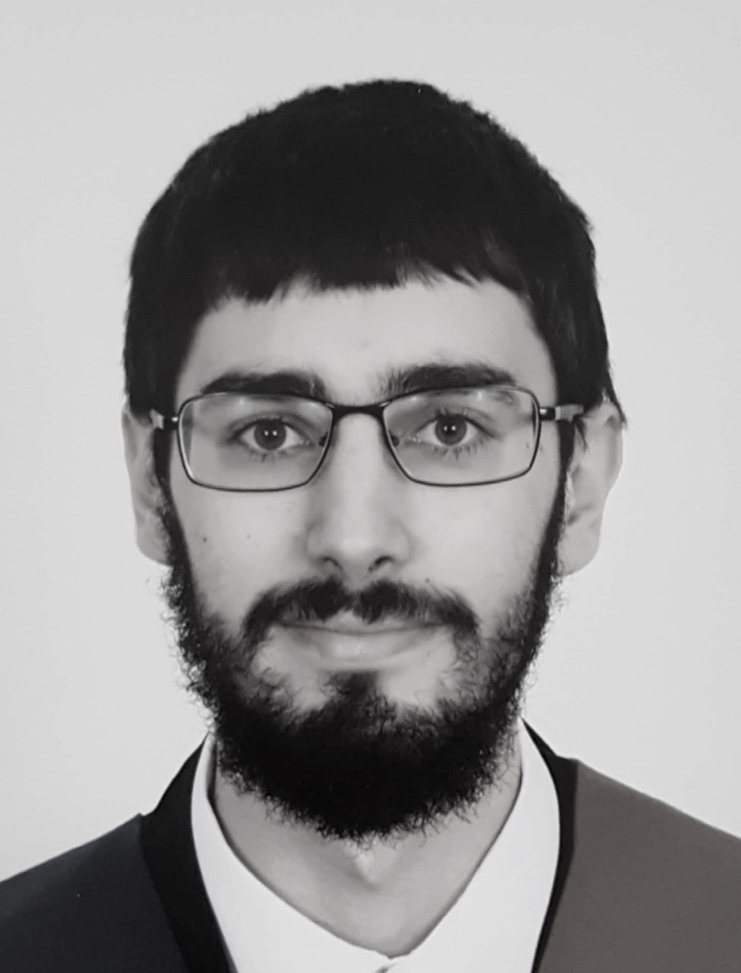
\includegraphics[width=\columnwidth]{img/dp_bn.jpeg}
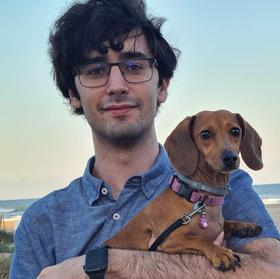
\includegraphics[width=\columnwidth]{img/dp_dog.jpeg}
Assistant Professor @ Universidad Autónoma de Madrid
  \section{contact}
    Daniel Perdices
    C-327
    EPS, UAM 
    Francisco Tomás y Valiente, 11 
    28049 Madrid (Spain)
    ~
    \href{mailto:daniel.perdices@uam.es}{daniel.perdices@uam.es}
    %\href{http://friggeri.net}{http://friggeri.net}
    %\href{http://facebook.com/adrien}{fb://adrien}
  \section{languages}
    Spanish native
    English advanced
    German intermediate 
    Japanese basic/intermediate
  \section{programming}
    Python (keras, pytorch, datascience libraries)
    C, C++, Go
    R, Matlab
    Spark, Hive
    JavaScript
    (ES6, angular, node.js)
\end{aside}


\section{interests}

network traffic analysis, service monitoring and management, data analysis, mathematical modelling, statistics, probability theory, stochastic processes, machine learning, deep learning, mathematical optimization, regularization techniques, distributed systems

\section{education}

\begin{entrylist}
%   \entry
%     {since 2009}
%     {Ph.D. {\normalfont candidate in Computer Science}}
%     {DNET/INRIA, LIP/ÉNS de Lyon}
%     {\emph{A Quantified Theory of Social Cohesion.}}
\entry
    {2020–2023}
    {Ph.D. in Computer Science and Telecomm.}
    {Universidad Autónoma de Madrid}
    {Grade \textit{sobresaliente cum laude} with honors \emph{(Premio extraordinario)}\\
    Research line: Data science, statistics \& AI applied to network monitoring \& web browsing privacy.\\
    Thesis: \href{https://repositorio.uam.es/bitstream/handle/10486/712298/perdices_burrero_daniel.pdf?sequence=1&isAllowed=y}{\emph{Smart Modeling Techniques for Network and Service Management}}\\
    Three month research intern at \href{https://smartdata.polito.it/}{\emph{SmartData@PoliTo - Interdepartamental centre of Politecnico di Torino}}
    }
\entry
    {2018–2020}
    {M.Sc. in ICT Research}
    {Universidad Autónoma de Madrid}
    {Specialization in Computational Intelligence\\
    Average grade 9.68, 6 courses (48 ECTS + 12 ECTS recognized) \\
    Machine Learning, Deep Learning, Parallel systems, Time information processing, Bayesian methods, Information retrieval \\
    M. Thesis: \href{https://repositorio.uam.es/bitstream/handle/10486/692579/perdices_burrero_daniel_tfm.pdf?sequence=1&isAllowed=y}{\emph{Network monitoring and performance assessment: from statistical models to neural networks}}\\%\emph{Partial Least Squares for Functional Data}
    }
  \entry
    {2018–2019}
    {M.Sc. in Mathematics and Applications}
    {Universidad Autónoma de Madrid}
    {Specialization in Applied mathematics\\
    Average grade 9.76, 5 courses (48 ECTS + 12 ECTS recognized)\\
    Statistics, Stochastic processes, signal processing, numerical methods\\
    M. Thesis: \href{https://dperdices.github.io/resources/Partial_Least_Squares_for_Functional_Data.pdf}{\emph{Partial Least Squares for Functional Data}}
    }
\entry
    {2013–2018}
    {B.Sc. in Mathematics}
    {Universidad Autónoma de Madrid}
    {First class honours.\\
    Average grade 9.26, 29 courses  (180 ECTS credits) with distinction. \\
    Statistics, mathematical optimization, functional analysis.\\
    Obtained in the program of the double degree in Computer Engineering and Mathematics (360 ECTS credits).\\
    Thesis: \tfg~(only available in Spanish).
    }
\entry
    {2013–2018}
    {B.Sc. in Computer Science/Engineering}
    {Universidad Autónoma de Madrid}
    {First class honours.\\
    Average grade 9.26, 29 courses  (180 ECTS) with distinction. \\
    Obtained in the program of the double degree in Computer Engineering and Mathematics (360 ECTS).\\
    Computer networks, machine learning, signal processing.\\
    Thesis: \tfg~(only available in Spanish).}
%   \entry
%     {2003}
%     {French Baccalauréat S. with honors}
%     {Lycée Louis le Grand, Paris}
%     {Specialization in mathematics and physics}
\end{entrylist}
\newpage
\section{publications}

%%% This piece of code has been commented by Karol Kozioł due to biblatex errors. 
\nocite{*}
\subsection{international peer-reviewed journal}
\begin{refsegment}
  \nocite{*}
  \printbibliography[sorting=chronological, type=article, notkeyword={spanish}, heading=none]
\end{refsegment}
\subsection{international peer-reviewed conferences/proceedings}
\begin{refsegment}
  \nocite{*}
  \printbibliography[sorting=chronological, type=inproceedings, notkeyword={spanish}, heading=none]
\end{refsegment}
\subsection{local peer-reviewed conferences/proceedings}
\begin{refsegment}
  \nocite{*}
  \printbibliography[sorting=chronological, type=inproceedings, keyword={spanish}, heading=none]
\end{refsegment}
\subsection{technical reports}
\begin{refsegment}
  \nocite{*}
  \printbibliography[sorting=chronological, type=report, heading=none]
\end{refsegment}

\section{experience}

\begin{entrylist}
\entry
    {10/2023}
    {Universidad Autónoma de Madrid (UAM) \hspace{1em} (Current) }
    {Assistant Prof.}
    {Area of Computer Architecture and Technologies. \\
    High Performance Computing and Networking research group.\\
    Department of Electronic and Communication Technologies.
    }
\entry
    {11/2020}
    {Universidad Autónoma de Madrid (UAM) \hspace{1em} (3 years) }
    {Researcher}
    {\emph{Spanish program for the formation of university lecturers \\
    Formación de Profesorado Universitario (FPU)}}
  \entry
    {10/2017}
    {Naudit HPCN, Madrid \hspace{1em} (3 years) }
    {Analyst \& Software Developer}
    {\emph{Network monitoring, data analysis and network architectures}}
\entry
    {02/2020}
    {UAM, Madrid \hspace{1em} (6 months) }
    {Adjunct Professor}
    {\emph{Teaching \& Research duties}}
\entry
    {06/2017}
    {Naudit HPCN, Madrid \hspace{1em} (3 months)}
    {Internship.}
    {\emph{Distributed systems, network monitoring and data analysis}}
    \entry
    {06/2016}
    {HPCN Research Group, UAM, Madrid \hspace{1em} (10 months) }
    {Research Internship.}
    {\emph{Passive measurements, Network modeling, OTT services}}{}
 
\end{entrylist}
\newpage

\section{management \& participation}

\begin{entrylist}
%   \entry
%     {since 2009}
%     {Ph.D. {\normalfont candidate in Computer Science}}
%     {DNET/INRIA, LIP/ÉNS de Lyon}
%     {\emph{A Quantified Theory of Social Cohesion.}}
\entry
    {2024-*}
    {Representative in Faculty Council (\textit{Junta de Centro})}
    {EPS-UAM}
    {Elective representative of non-tenured professors and researchers (\textit{PDI no permanente}) in the Faculty Council
    }
\entry
    {2023-*}
    {Permanent member of Department Council (\textit{CD de TEC)}}
    {TEC-EPS-UAM}
    {Permanent member (as Ph.D.) of the Electronics and Communication Technologies Department Council (Consejo del Departamento de Tecnología Electrónica y de las Comunicaciones).}
\entry
    {2021-2023}
    {Representative in Faculty Council (\textit{Junta de Centro})}
    {EPS-UAM}
    {Elective representative of Ph.D candidates (\textit{PDI en Formación}) in the Faculty Council.
    }
\entry
    {2021-2023}
    {Representative in Department Council (\textit{CD de TEC)}}
    {TEC-EPS-UAM}
    {Elective representative of Ph.D candidates (\textit{PDI en Formación}) in the Electronics and Communication Technologies Department Council (Consejo del Departamento de Tecnología Electrónica y de las Comunicaciones).}
\end{entrylist}
\vspace{-2em}
\section{languages}
\subsection{accreditations}


\begin{itemize}
\setlength\itemsep{-0.4em}
    \item Spanish \hfill {\addfontfeature{Color=lightgray} Native}
    \item English \hfill {\addfontfeature{Color=lightgray} C2 CEFR}
    \begin{itemize}
        \item C2 accreditation 
        
        Certificate in Advanced English (Cambridge)
        
        Grade A - 203/210 
    \end{itemize}

    \item German \hfill {\addfontfeature{Color=lightgray} B1 CEFR}
    \begin{itemize}
        \item B1 Spanish official language school accreditation 
    \end{itemize}
    \item Japanese \hfill {\addfontfeature{Color=lightgray} B1.1/B1.2 CEFR}
    \begin{itemize}
        \item Japanese Language Proficiency Test N4
    \end{itemize}
\end{itemize}

\subsection{courses}
    \begin{itemize}
    \setlength\itemsep{-0.4em}
    \item English
    \begin{itemize}
        \item C1 Advanced preparation course (60 hours) \hfill %{\addfontfeature{Color=lightgray} C1.2 CEFR}
        \item B2 accreditation preparation course (60 hours)
    \end{itemize}
    \item German
    \begin{itemize}
        \item B1 course at Sprachcaffe Frankfurt, Germany
        \item B1.1 course at Spanish Official Language School
        \item B1.2 course at Spanish Official Language School
    \end{itemize}
    \item Japanese \hfill 
    \begin{itemize}
        \item B1.1/B1.2 course at Universidad Complutense de Madrid (75 hours)
        \item A2.2 course at Universidad Complutense de Madrid (60 hours)
        \item A2.1 course at Universidad Complutense de Madrid (60 hours)
        \item A1.2 course at Universidad Complutense de Madrid (75 hours)
        \item A1.1 course at Universidad Complutense de Madrid (75 hours)
    \end{itemize}
\end{itemize}

%\newpage

\section{extra education}
\begin{entrylist}
%   \entry
%     {since 2009}
%     {Ph.D. {\normalfont candidate in Computer Science}}
%     {DNET/INRIA, LIP/ÉNS de Lyon}
%     {\emph{A Quantified Theory of Social Cohesion.}}
\entry
    {06/2024}
    {Intellectual property: practical aspects for university lecturers}
    {UAM}
    {Teacher training program course\\
    1 ECTS
    }
\entry
    {02/2024}
    {How to evaluate learning outcomes.}
    {UAM}
    {Teacher training program course\\
    1 ECTS
    }
\entry
    {01/2024}
    {The concept of competence and competence training.}
    {UAM}
    {Teacher training program course\\
    1 ECTS
    }
\entry
    {12/2023}
    {Design and planning of the teaching-learning process in the context of a subject. Preparation of the syllabus.}
    {UAM}
    {Teacher training program course\\
    2 ECTS
    }
\entry
    {11/2023}
    {Authority and leadership. Communication in the classroom.}
    {UAM}
    {Teacher training program course\\
    1 ECTS
    }
    
\entry
    {07/2021}
    {Digital Competences for University Lecturers. Creation of Educational Resources I.}
    {UAM}
    {Teacher training program course\\
    2 ECTS (25 hours)
    }
    
\entry
    {07/2021}
    {Edition of audiovisual educational resources: image processing, screen recording and video editing.}
    {UAM}
    {Teacher training program course\\
    2 ECTS (25 hours)
    }

\entry
    {07/2021}
    {Digital Competences for University Lecturers. Tools for teaching from home in MS Teams environment.}
    {UAM}
    {Teacher training program course\\
    2 ECTS (25 hours)
    }
    
\entry
    {07/2020}
    {DL0101EN: Deep Learning Fundamentals with Keras}
    {IBM}
    {edX course\\
    {\href{https://courses.edx.org/certificates/6766636dcd5a4a2293edef7d424a24a2}{Verified certificate: 6766636dcd5a4a2293edef7d424a24a2}}
    }
\entry
    {07/2020}
    {DL0110EN: Deep Learning with Python and PyTorch}
    {IBM}
    {edX course\\
    {\href{https://courses.edx.org/certificates/86c87963b1c04a23a2d6f63140f53beb}{Verified certificate: 86c87963b1c04a23a2d6f63140f53beb}}
    }
  \entry
    {09/2020}
    {DL0120EN: Deep Learning with Tensorflow}
    {IBM}
    {edX course\\
    {\href{https://courses.edx.org/certificates/b3b1e106872d468b86fbeb4d42bb5db7}{Verified certificate: b3b1e106872d468b86fbeb4d42bb5db7}}
    } 
    \entry
    {08/2020}
    {PH525.1x: Statistics and R}
    {Harvard University}
    {edX course\\
    {\href{https://courses.edx.org/certificates/dc3c5dcde68d44afbaa8dbdfd46c72da}{Verified certificate: dc3c5dcde68d44afbaa8dbdfd46c72da}}
    }
    
\entry
    {08/2020}
    {PH525.2x: Introduction to Linear Models and Matrix Algebra}
    {Harvard U.}
    {edX course\\
    {\href{https://courses.edx.org/certificates/7b43079626ee407eb65e28b03ae937bb}{Verified certificate: 7b43079626ee407eb65e28b03ae937bb}}
    } 
\entry
    {08/2020}
    {PH525.3x: Statistical Inference and Modeling for High-throughput Experiments}
    {Harvard University}
    {edX course\\
    {\href{https://courses.edx.org/certificates/19a6232d263d479389809a306017fe56}{Verified certificate: 19a6232d263d479389809a306017fe56}}
    } 
    \entry
    {08/2020}
    {PH525.4x: High-Dimensional Data Analysis}
    {Harvard University}
    {edX course\\
    {\href{https://courses.edx.org/certificates/0d825e7908f24419825a0ca21dd09750}{Verified certificate: 0d825e7908f24419825a0ca21dd09750}}
    } 
    \entry
    {08/2020}
    {XSeries: Data Analysis for Life Science}
    {Harvard University}
    {edX XSeries program\\
    {\href{https://credentials.edx.org/credentials/70a313930dfa4846b4047abb6b5ed018/}{Verified certificate: 70a313930dfa4846b4047abb6b5ed018}}
    }
    \entry
    {08/2020}
    {Professional Certificate: Data Analysis for Life Science}
    {Harvard University}
    {edX Professional certificate\\
    {\href{https://credentials.edx.org/credentials/cb1e72a648cb4987958d1836b401cf81/}{Verified certificate: cb1e72a648cb4987958d1836b401cf81}}
    }
\end{entrylist}



%\subsection{theses}
%\begin{refsection}
%  \nocite{*}
%  \printbibliography[sorting=chronological, type=thesis, heading=none]
%\end{refsection}
\section{teaching}
\begin{entrylist}
\entry{2019-2023}{DOCENTIA-UAM}{Grade A}{
17th program for the evaluation of teaching activities.\\
Grade obtained: A (94.97).
}
\entry{2023-24}
{Computer Networks}
{B.Sc. in Data Science and Engineering}
{Laboratory sessions. Assistant Professor. Competences: network stack, access layer, Ethernet, ARP, network layer, IP, TCP, UDP, ICMP, application layer, HTTP, DNS. 
}
\entry{2023-24}
{Network Architecture II}
{B.Eng. in Telecommunication Technology and Services}
{Laboratory sessions. Assistant Professor. Competences: access layer, wireless technologies, ARP, Ethernet, IEEE 802.11, queuing theory, security, TLS. %26 hours (13 sessions).
}
\entry{2023-24}
{High Performance Computing}
{B.Eng. in Computer Science}
{Theory \& Laboratory sessions. Assistant professor. Competences: CPU vectorization, parallelism algorithms, HPC architectures, GPGPU, CUDA, Apache Hadoop, Apache Spark, Cloud computing, Kubernetes. 
}
\entry{2022-23}
{Computer Networks I}
{B.Eng. in Computer Science}
{Laboratory sessions. Teaching assistant/collaborator. Competences: network stack, access layer, Ethernet, ARP, network layer, IP, TCP, UDP, ICMP. 
}
\entry{2022-23}
{High Performance Computing}
{B.Eng. in Computer Science}
{Laboratory sessions. Teaching assistant/collaborator. Competences: CPU vectorization, parallelism algorithms, HPC architectures, GPGPU, CUDA, Apache Hadoop, Apache Spark, Cloud computing, Kubernetes. 
}
\entry{2021-22}
{Computer Networks I}
{B.Eng. in Computer Science}
{Laboratory sessions. Teaching assistant/collaborator. Competences: network stack, access layer, Ethernet, ARP, network layer, IP, TCP, UDP, ICMP. %26 hours (13 sessions).
}
\entry{2021-22}
{Computer Architecture}
{B.Eng. in Computer Science (English)}
{Laboratory sessions. Teaching assistant/collaborator. Competences: hardware design languages, processor design, performance assessment, cache performance, parallelism, OpenMP. %26 hours (13 sessions).
}
\entry{2020-21}
{Computer Architecture}
{B.Eng. in Computer Science}
{Laboratory sessions. Teaching assistant/collaborator. Competences: hardware design languages, processor design, performance assessment, cache performance, parallelism, OpenMP. %26 hours (13 sessions).
}
\entry{2019-20}
{Network Architecture I}
{B.Eng. in Telecommunication Technology and Services}
{Laboratory sessions. Teaching assistant/collaborator. Competences: network stack, network architecture and design, application layer (HTTP, DNS programming), transport layer (TCP, UDP), network layer, network traffic dissection, Wireshark, tshark. %26 hours (13 sessions).
}
\entry{2019-20}
{Network Architecture II}
{B.Eng. in Telecommunication Technology and Services}
{Laboratory sessions. Adjunct Professor. Competences: access layer, wireless technologies, ARP, Ethernet, IEEE 802.11, queuing theory, security, TLS. %26 hours (13 sessions).
}
\entry{2019-20}
{Parallel System Architecture}
{B.Eng. in Computer Science}
{Laboratory sessions. Adjunct Professor (Laboratory coordinator). Competences: MPI, Sun Grid Engine, OpenMP, parallelism algorithms, HPC architectures, GPGPU, CUDA, Apache Hadoop, Apache Spark. %26 hours (13 sessions).
}
\entry{2019-20}
{End-of-degree thesis}
{B.Eng. in Computer Science \& B.Sc. in Mathematics}
{Advisor as an industrial project. Title: "Interacción con usuario para reporte y diagnóstico de incidencias" (only available in Spanish)
}
\end{entrylist}

\section{participation in research projects}
\vspace{-1em}
\begin{entrylist}
\entry{2025-*}
{LINO}
{Comunidad de Madrid}
{\textbf{Principal Investigator} in "LINO: A LLM Integrated in Network Operation (SI4/PJI/2024-00221)" as an assistant professor.
}
\entry{2025-*}
{RAMONES-CM}
{Comunidad de Madrid}
{Participation in "RAMONES-CM - Research in Advanced Monitoring and Optimization for Next-gen post-quantum Encryption and cyberSecurity" as an assistant professor.
}
\entry{2021-2024}
{AGILEMON}
{Spanish State Agency of Research}
{Participation in "AGILEMON: Hacia un nuevo paradigma de análisis de rendimiento agile para servicios (AEI PID2019-104451RB-C21)" as a FPU researcher.
}
\entry{2017-2020}
{METRO-HAUL}
{European Comission}
{Collaboration in "METRO-HAUL: METRO High bandwidth, 5G Application-aware optical network, with edge storage, compUte and low Latency (European Comission, Project Id. 761727)" as a collaborator in naudit.
}
\entry{2017-2018}
{TRAFICA}
{Spanish Ministry of Science and Innovation}
{Collaboration in  "Tráfica: Análisis de tráfico para inteligencia operativa (Programa Estatal de Investigación, Desarrollo e Innovación Orientada a los Retos de la Sociedad, TEC2015-69417-C2-1-R.)" as holder of the collaboration scholarship of the Spanish Ministry of Education, Sports and Culture.
}
\end{entrylist}
\vspace{-2em}
\section{awards}
\hspace{-5em}\vspace{-2.5em}
\begin{entrylist}
\entry{2023}
{Distinction in Ph.D. studies}
{Universidad Autónoma de Madrid}
{Given as a recognition to the best Ph.D. record of year 2023 in the PhD Program of Computer and Telecommunication Engineering}
\entry{2021}
{Student Travel Grant for CNSM 2021}
{CNSM community}
{Student Travel Grant to attend the 17th International Conference on Network and Service Management (CNSM) 2021 held in Izmir, Turkey (Online), where I presented~\cite{cnsm2021} in the MC Session 4.}
\entry{2018}
{First Class Honours}
{Universidad Autónoma de Madrid}
{Given as a recognition to the performance in the Double degree in Computer Engineering and Mathematics}
\entry{2018}
{Best Student Paper Award at CNSM 2018}
{IFIP - IEEE ComSoc}
{Best Student Paper Award at the 14th International Conference on Network and Service Management (CNSM) 2018 held in Rome, Italy. It was given to my paper~\cite{cnsm2018}.}
\entry{2018}
{Student Travel Grant for CNSM 2018}
{IFIP}
{Student Travel Grant to attend the 14th International Conference on Network and Service Management (CNSM) 2018 held in Rome, Italy, where I presented~\cite{cnsm2018} in the Technical Session 1.}
\entry{2017-2018}
{Collaboration scholarship}
{Spanish Ministry of Education, Culture and Sports}
{Given to carry out a project at the High Performance Computing and Networking research group of UAM (supervisor:  Prof. Jorge E. López de Vergara).}
\entry{2017-2018}
{University excellence scholarship}
{Madrid's Autonomous Community }
{Given due to an excellent academic record during the previous year.}
\entry{2016-2017}
{University excellence scholarship}
{Madrid's Autonomous Community }
{Given due to an excellent academic record during the previous year.}
\entry{2015-2016}
{University excellence scholarship}
{Madrid's Autonomous Community }
{Given due to an excellent academic record during the previous year.}
\entry{2014-2015}
{University excellence scholarship}
{Madrid's Autonomous Community }
{Given due to an excellent academic record during the previous year.}
\entry{2014}
{Best academic record of first year}
{Universidad Autónoma de Madrid }
{Given due to the performance in the first year of my bachelor's degree.}
\entry{2013-2014}
{University excellence scholarship}
{Madrid's Autonomous Community }
{Given due to an excellent result in the university access exam.}
\entry{2011}
{Honorific mention at compulsory education}
{Madrid's Autonomous Community }
{Given due to an outstanding academic record during compulsory secundary education.}
\end{entrylist}
%•	Diploma en Curso de Voluntariado, Comunidad de Madrid. Junio 2014.
%•	Diploma con Matrícula de Honor por su rendimiento en los estudios de Bachillerato finalizados en el curso 2012/2013.
%•	Diploma de participación en CAMPUS CIENTIFICO de Verano 2012, Proyecto “Criptografía y números primos” en la Universidad  de Sevilla. Julio 2012.
%•	1º Premio Bachillerato, V Olimpiada Matemática, X Semana Cultural Fundación Caldeiro, Curso 2011/2012.


%%% This piece of code has been commented by Karol Kozioł due to biblatex errors. 
% 
%\printbibsection{article}{article in peer-reviewed journal}
%\begin{refsection}
%  \nocite{*}
%  \printbibliography[sorting=chronological, type=inproceedings, title={international peer-reviewed conferences/proceedings}, notkeyword={france}, heading=subbibliography]
%\end{refsection}
%\begin{refsection}
%  \nocite{*}
%  \printbibliography[sorting=chronological, type=inproceedings, title={local peer-reviewed conferences/proceedings}, keyword={france}, heading=subbibliography]
%\end{refsection}
%\printbibsection{misc}{other publications}
%\printbibsection{report}{research reports}


\end{document}
